\documentclass[a4paper,12pt]{article}

\topmargin -0.80cm \headheight 0.40cm \textwidth 15truecm
\textheight 24.4truecm

\usepackage[dvips]{graphics}
\usepackage[ansinew]{inputenc}
\usepackage[preprint]{epsfig}
\usepackage{setspace}
\usepackage{lineno}
\usepackage{graphicx}
\usepackage{cite}
\usepackage{lscape}
\usepackage{amsfonts}

\begin{document}

\singlespacing

\newcommand{\cao}{\c{c}\~ao }
\newcommand{\coes}{\c{c}\~oes }
\newcommand{\caO}{\c{c}\~ao}
\newcommand{\coeS}{\c{c}\~oes}
\newcommand{\CAO}{\c{C}\~AO}
\newcommand{\COES}{\c{C}\~OES}
\newcommand{\cc }{\c{c}}
\newcommand{\CC }{\c{C}}
\newcommand{\y }{\'{\i}}
\def\gsim{\raise0.3ex\hbox{$\;>$\kern-0.75em\raise-1.1ex\hbox{$\sim\;$}}}

\def\binom#1#2{{#1\choose#2}}

%\begin{center}
%{\Large {\bf Letter to the Editor}}
%\end{center}
%\vskip 0.7cm

\vskip 1cm
\begin{center}
{\Large {\bf

A numerical study on the regularity of $d$-primes via informational
entropy and visibility algorithms

}}

\vskip 0.7cm

{\large {\rm B.L. Mayer$^{\rm{(a,1)}}$ and L.H.A.
Monteiro$^{\rm{(a,b,2)}}$}}


\vskip 0.5cm {\small

(a) Universidade Presbiteriana Mackenzie,

\vskip 0.05cm PPGEEC, S\~ao Paulo, SP, Brazil

\vskip 0.5cm (b)  Universidade de S\~ao Paulo,

\vskip 0.05cm Escola Polit\'ecnica, S\~ao Paulo, SP, Brazil


\vskip 0.5cm

\vskip 0.5cm (1) bleemayer@gmail.com

\vskip 0.1cm (2) luizm@mackenzie.br, luizm@usp.br }

\end{center}

\vskip 2cm

\begin{center}
{\it Corresponding author:}

\vskip 0.05cm Luiz Henrique Alves Monteiro

\vskip 0.05cm Universidade Presbiteriana Mackenzie

\vskip 0.05cm Escola de Engenharia

\vskip 0.05cm Rua da Consola\caO, n.896

\vskip 0.05cm 01302-907, S\~ao Paulo, SP, Brazil

\vskip 0.05cm E-mail addresses: luizm@mackenzie.br, luizm@usp.br

\vskip 0.05cm Telephone number: (55)(11)2114-8711

\vskip 0.05cm Fax number: (55)(11)2114-8600

\vskip 1cm ORCID ID: 0000-0002-2309-1254
\end{center}


\newpage


\doublespacing
\begin{center}
{\bf Abstract}
\end{center}

Let a $d$-prime be a positive integer number with $d$ divisors. From
this definition, the usual prime numbers correspond to the
particular case $d=2$. Here, the seemingly random sequence of gaps
between consecutive $d$-primes is numerically investigated. First,
the variability of the gap sequences for $d \in \{2,3,...,11\}$ is
evaluated by calculating the informational entropy. Then, these
sequences are mapped into graphs by employing two visibility
algorithms. Computer simulations reveal that the degree distribution
of most of these graphs follows a power law.
%; therefore, they are scale free.
Conjectures on how some
topological features of these graphs depend on $d$ are proposed.
%A consequence of this study is the following
%conjecture: $d$-primes are generated by deterministic rules.



\vskip 0.4cm \noindent {\it Keywords:} $d$-prime, informational
entropy, power law, time series, visibility graph.

\newpage

\section{Introduction}


Prime numbers, the building blocks of any positive integer,
fascinate math lovers \cite{a44,a66}. From a purely theoretical
perspective, primes are crucial for understanding the properties of
numbers \cite{a44,a66}. From an applied science perspective, primes
have been used in cryptographic keys \cite{a65}, can be found in the
life cycles of cicadas \cite{a48}, and characterize the energy
spectrum of chaotic quantum systems \cite{a59}.

Since 300 BC, the irregular distribution of primes throughout the
sequence of natural numbers has been extensively investigated.
Giants as Chebyshev, Dirichlet, Eratosthenes, Erd\"os, Euclid,
Euler, Fermat, Gauss, Legendre, and Riemann analyzed this matter
\cite{a44,a66}. To get some insight on this distribution, the
statistical properties of the gaps between consecutive primes
\cite{a64,a03}, second order gaps (the gaps between these gaps), and
higher order gaps \cite{a05,a02} have also been examined. The
distribution of primes has also been studied by using graphs. For
instance, consider that primes are the nodes of a graph. Since any
even number can be written as the sum of two primes, then a pair of
nodes is linked in this graph if it represents the sum of a given
even number \cite{a04}. In another graph-based approach, the natural
numbers are the nodes and there is a connection between two nodes if
they share a common prime divisor \cite{a16}. Graphs are also used
in this work.

Assume that a $d$-prime is a positive integer with $d$ divisors.
Therefore, the usual prime numbers correspond to the case $d=2$. In
this work, the frequency of the gaps between $d$-primes is
computationally analyzed. First, the difference of successive
$d$-primes is calculated for $d \in \{2,3,...,11\}$ and the gap
sequences thereby obtained are considered as discrete time series.
%;that is, a discrete-time dynamical system.
To evaluate their variability, the informational entropy \cite{a301}
of these series is computed. In addition, these series are
transformed into undirected graphs by applying two visibility
algorithms \cite{a14,a13}. The degree distribution and the average
degree of these graphs
%derived from the
%first order difference of consecutive $d$-primes for $d=2,3,4,5$
are determined and compared. These are the main contributions of
this work, which are described in the next section.

The aim of this study based on $d$-primes is to understand how the
gap sequences depend on $d$.
%This study can provide an alternative
%way of investigating the occurrence of the usual primes, which are
%the factors of any $d$-prime with $d>2$.
The proposed approach can
be used to analyze other sequences of numbers found in nature
\cite{a300}, such as the energy levels of atomic nuclei  and the
quantum space-time structure \cite{x1}.


\section{Methodology and numerical results}


Let a $d$-prime be defined as a positive integer $p_d$ greater than
1 that is divisible by 1, the number itself, and $d-2$ (smaller)
positive integers. Thus, a $d$-prime has exactly $d$ distinct
divisors. For instance,
%the number 10 is a 4-prime because its divisors are 1, 2, 5, and 10;
%the number 11 is a 2-prime because its divisors are 1 and 11;
the number 12 is a 6-prime because its (six) divisors are 1, 2, 3,
4, 6, and 12. A $d$-prime with $d>2$ is usually called a composite
number \cite{a44,a66}. Note that the 2-primes are just the usual
primes. Thus, $d$-prime is a naive generalization of the concept of
prime number.

Let $p_d(n)$ be the $n$-th $d$-prime, with $n \in \mathbb{N}^*$. For
instance, $p_3(4)$ is the fourth 3-prime, which is equal to 49.
Table 1 presents a list of the first $d$-primes for $d \in
\{2,3,...,11\}$. Let $x_d(n)=p_d(n+1)-p_d(n)$ be the gap between
consecutive $d$-primes. For instance, $x_5(1)=65$, because
$p_5(2)=81$ and $p_5(1)=16$. Note that the sequence $x_d(n)$ can be
taken as a time series, in which $n$ corresponds to the time
variable. Table 2 shows the first numbers of the series $x_d(n)$ for
$d \in \{2,3,...,11\}$.

In order to evaluate the variability of the series $x_d$ for $d \in
\{2,3,...,11\}$, the informational entropy $H$ \cite{a301} was
computed. This entropy has been calculated, for instance, in
investigations on the dynamics of biological \cite{a305} and social
systems \cite{a302}. Its normalized value, denoted by $\Delta$, is
given by:
\begin{equation}
\Delta = \frac{H}{H_{max}}
\end{equation}


\noindent The entropy $H=-\sum_{i=1}^q p_i \ln p_i$ and its maximum
value $H_{max}=\ln q$ (obtained in the case of $p_i=1/q$ for
$i=1,...,q$ \cite{a301}) are calculated by taking $p_i$ as the
relative frequency of occurrence of a distinct $x_d$. In these
expressions, $q$ is the number of distinct values of $x_d$.

As the next step, the time series $x_d(n)$ were converted into
undirected graphs by using two visibility algorithms \cite{a14,a13}.
These algorithms have been employed, for instance, in the analysis
of stock indices \cite{a94} and electroencephalography recordings
\cite{b01}. Here, in the visibility graphs, each node represents a
distinct value of $x_d$.

Consider that $n_a < n_i < n_b$. In the natural visibility (NV)
graph \cite{a14}, the nodes corresponding to $x_d(n_a)$ and
$x_d(n_b)$ are connected if any intermediate point $(n_i,x_d(n_i))$
in the time series satisfies the inequality:
\begin{equation}
x_d(n_i) < x_d(n_a) + \left( x_d(n_b)-x_d(n_a) \right) \left(
\frac{n_i-n_a}{n_b-n_a} \right)
\end{equation}

\noindent Thus, these nodes are connected if there is a straight
line joining $(n_a,x_d(n_a))$ and $(n_b,x_d(n_b))$ in the plot
$x_d(n) \times n$, provided that any intermediate point
$(n_i,x_d(n_i))$ is below such a line. For instance, the four first
points of the sequence $x_3(n)$ shown in Table 2 are $x_3(1)=5$,
$x_3(2)=16$, $x_3(3)=24$, and $x_3(4)=72$. There is a connection
between the nodes corresponding to $x_3=16$ and $x_3=72$, because
the intermediate datum $x_3=24$ is below the straight line linking
these points in the plot $x_3(n) \times n$; that is, because
$x_3(3)= 24 < x_3(2) + (x_3(4)-x_3(2)) (3-2)/(4-2)= 16 + (72-16)/2 =
44$.
%Thus, the nodes 16 and 72 can see each other.
Also, note that there is not a connection between the nodes $x_3=5$
and $x_3=24$, because $x_3(2)=16 > x_3(1) +
(x_3(3)-x_3(1))(2-1)/(3-1) = 5 + (24-5)/2 = 14.5$. In this case, the
datum (2,16) is high enough to prevent the data (1,5) and (3,24)
from seeing each other.
%(by considering only the beginning of the plot $x_3(n) \times n$).


In the horizontal visibility (HV) graph  \cite{a13}, the nodes
associated with $x_d(n_a)$ and $x_d(n_b)$ are connected if:
\begin{equation}
\left\{ x_d(n_a),x_d(n_b) \right\} > x_d(n_i)
\end{equation}

\noindent with $n_a < n_i < n_b$. Thus, these nodes are connected if
any intermediate point $(n_i,x_d(n_i))$ in the plot $x_d(n) \times
n$ is below the horizontal line joining $(n_a,x_d(n_a))$ and
$(n_b,x_d(n_b))$. In the HV graph built from the beginning of the
sequence $x_3(n)$, the nodes corresponding to $x_3=16$ and $x_3=72$
are not connected, because $x_3(2)=16<x_3(3)=24$; that is, $(2,16)$
and $(4,72)$ can not see each other because $(3,24)$ is high enough
to block their horizontal visibility. Thus, $x_3=16$ and $x_3=72$
are connected in the NV graph, but they are not connected in the HV
graph.

Numerical experiments were performed by taking $n=1,2,...,10000$;
that is, the first 10000 $d$-primes for each value of $d$. From
these 10000 $d$-primes, 9999 values of $x_d(n)$ were computed. The
values corresponding to $n=1,2,9998, 9999$ were discarded, in order
to neglect the initial transient ($n=1,2$) and the effects of
truncation ($n=9998,9999$).

The normalized entropy $\Delta$ was computed by using Eq. (1). As
Table 3 shows, $\Delta=1$ for $d=5, 7$, and $11$, because there is
no repeated value of $x_d$ in the corresponding sequences.
 For $d=3$ and
$d=9$, $\Delta \simeq 1$; for $d$ even, $\Delta \approx 0.7$. Hence,
for $d \in \{2,3,...,11\}$, $d$ odd favors equiprobable values of
$p_i$ more than $d$ even.

From the gap sequences $x_d(n)$ for $d \in \{2,3,...,11\}$,
undirected visibility graphs were built by using Eqs. (2) and (3).
Then, the corresponding degree distributions $P(k)$ and the average
degree $\langle k \rangle$ were determined. Recall that the degree
of a node is the number of edges connected to this node \cite{b02}.
 Recall also that the degree distribution
expresses how the percentage $P(k)$ of nodes with degree $k$ varies
with $k$ \cite{b02}. Usually, $P(k)$ is interpreted as the
probability of randomly picking a node \mbox{with degree $k$.}

Figures 1 and 2 exhibit the log-log plot of $P(k)$ for NV and HV
graphs, respectively, for $d \in \{2,3,...,11\}$. Observe that most
$P(k)$ decays as a power law in these plots. Power laws have been
found in the distribution of prime gaps \cite{li1} and in a myriad
of contexts, such as psychiatric ward \cite{b04} and financial
crashes \cite{a99}. Here, $P(k)$ is proportional to $k$ taken to the
power $-\gamma$; that is, $P(k) = A k^{-\gamma}$, in which $A$ is
the proportionality constant. In a log-log plot, $\log P(k) = \log A
- \gamma \log k$; thus, the power law dependence is transformed into
a linear relation between $\log P(k)$ and $\log k$. At least as a
first approximation, this relation can be taken as linear in most
plots shown in both figures; that is, a power-law form for $P(k)$
can be considered a plausible model for these plots. Possible
exceptions are the NV plots for $d=\{7,11\}$.

%In the other NV plots and in all HV plots, the fluctuations observed
%around the fitted straight lines can be effects of the finite size
%of the gap sequences $x_d(n)$ used in the numerical experiments
%\cite{li2}.

Tables 4 and 5 present $A$, $\gamma$, and  $\langle k \rangle$ for
the 20 graphs.
%The values of $A$ and $\gamma$ were determined
%by using the method of least squares  \cite{b03}.
The average degree $\langle k \rangle$ for the HV graphs are smaller
than for the NV graphs, because HV graphs are subgraphs of the
corresponding NV graphs. For the NV graphs, $\langle k \rangle
\approx 6$, with the exception of $d=\{5,7,11\}$, which present
higher values. For the HV graphs, $\langle k \rangle > 3.90$ for $d$
odd and $\langle k \rangle < 3.90$ for $d$ even. Note also that the
values of $A$ and $\gamma$, determined from a least-squares fitting
\cite{b03}, present smaller variability for the HV graphs than for
the NV graphs. In addition, for the NV graphs, $\gamma \simeq 1.1$;
for the HV graphs, $\gamma \simeq 1.7$.

From the numerical experiments reported in this work, the following
relations were found: $p_3(n)=(p_2(n))^2$, $p_5(n)=(p_2(n))^4$,
$p_7(n)=(p_2(n))^6$, and $p_{11}(n)=(p_2(n))^{10}$; thus, 3-primes,
5-primes, 7-primes, and 11-primes are just powers of prime numbers
with power 2, 4, 6, and 10 respectively. However, no relation
between $p_2(n)$ and $p_j(n)$ with $j=\{4,6,8,9,10\}$ was found;
that is, no relation was found between prime numbers and $d$-primes
when $d$ is not prime.



\section{Discussion and Conclusion}

The absence of a discernible pattern in the sequence of prime
numbers has historically hampered the derivation of a formula for
correctly generating such a sequence \cite{a44,a66}. The analytical
generation of $d$-primes, with $d>2$, can be an even more
challenging task, mainly if $d$ is not prime. Here, the distribution
of the gaps between $d$-primes was examined by using a complexity
measure and two visibility graphs.

As shown in Table 3, $\Delta \simeq 1$ for $d=\{3,5,7,9,11\}$,
because repetitions in the sequences of $x_d$ are absent or rare;
that is, these sequences are aperiodic. In addition, $\Delta \approx
0.7$ for $d=\{2,4,6,8,10\}$; thus, the variability of the gap
lengths for $d$ even is lower than for $d$ odd. Therefore, a
possible conjecture is: the normalized entropy $\Delta$
distinguishes $d$ even ($\Delta \approx 0.7$) from $d$ odd ($\Delta
\simeq 1$).


As shown in Figures 1 and 2 and Tables 4 and 5, most degree
distributions $P(k)$ of the visibility graphs built from the
differences between successive $d$-primes for $d \in \{2,3,...,11\}$
approximately follows a power law written as $P(k)=A k^{-\gamma}$.
Fluctuations observed around the fitted straight lines shown in both
figures can be effects of the finite size of the gap sequences
$x_d(n)$ used in the numerical experiments \cite{li2}. Recall that
power-law distributions in the connectivity are associated with
complex networks known as scale-free \cite{li2,a81,a83}. Scale
invariance in the degree distribution implies self-similarity; that
is, the $P(k)$ of renormalized networks, obtained by a
coarse-graining procedure \cite{a400}, also follows a power law.
Note that the value of $\gamma$ in the NV and HV plots is not a good
parameter to show the influence of the value of $d$ on the networks
derived from the gap sequences; however, $\langle k \rangle$ can
highlight this influence: in NV plots, for $d$ that is prime,
$\langle k \rangle$ increases with $d$; for $d$ that is not prime,
$\langle k \rangle \approx 6$; in HV plots, $\langle k \rangle >
3.90$ for $d$ odd and $\langle k \rangle < 3.90$ for $d$ even.
Therefore, another possible conjecture is: $\langle k \rangle$ in NV
plots distinguishes $d$ that is prime from $d$ that is not prime;
$\langle k \rangle$ in HV plots distinguishes $d$ odd from $d$ even.

It is well known that, for HV graphs obtained for periodic sequences
of period $T$ (without repeated number within a period), the average
degree is given by $\langle k \rangle = 4[1-(1/(2T)]$ \cite{a310}.
As a consequence, for aperiodic series, $\langle k \rangle = 4$
(because $T \to \infty$). According to Table 5, this is the
approximate value of $\langle k \rangle$ found for $d$-primes with
$d$ odd, which is in agreement with the value of $\Delta$ presented
in Table 3. It is also well known that, for an uncorrelated random
sequence, the HV graph has $P_{rand}(k)= (1/3)(2/3)^{k-2}$
\cite{a310}. Therefore, deviations from this degree distribution
reveal that the studied sequence was not generated by an
uncorrelated random process. The straight line corresponding to
$P_{rand}(k)$ is shown as a dotted line in Figure 2. Note that
$P(k)$ for $d$-primes has smaller slope than the slope of
$P_{rand}(k)$. This smaller slope and $\langle k \rangle = 4$ can be
features of chaotic sequences \cite{a310}.



%As shown in Figs. 1-4 and Table 4, the degree distributions $P(k)$
%of the visibility graphs built from the differences between
%successive $d$-numbers for $d \in \{2,3,...,9\}$ obey a power law
%written as $P(k)=A k^{-\gamma}$. Power-law distributions in the
%connectivity are associated with complex networks known as
%scale-free \cite{a81,a83}, and scale-free networks derived from
%visibility algorithms have been associated with chaotic behavior
%\cite{a14,a13}. Chaos arises from deterministic systems \cite{b02}.
%Therefore, our results support the following conjecture: the gaps
%between consecutive $d$-primes are generated by deterministic
%equations. Consequently, the $d$-primes themselves are generated by
%deterministic equations. In fact, 3-primes, 5-primes, and 7-primes
%are directly computed from 2-primes; however, for $d \in
%\{2,3,...,9\}$, the relations between $d$-primes and 2-primes when
%$d$ is not a 2-prime are not yet evident.

%Also,  a formula for generating the exact sequence of usual primes
%remains to be found.

%In short: for $d \in \{2,3,...,9\}$, the values of normalized
%entropy $\Delta$ show that the variability in the gap length of
%$d$-primes is higher for $d$ odd than for $d$ even. In addition, the
%topological properties of the visibility graphs built from the gap
%frequencies suggest that these gaps can be generated by
%deterministic rules.

A final comment about the generation of $d$-primes by deterministic
equations: when $d$ is prime, then $p_d(n)=(p_2(n))^{d-1}$; however,
the way of obtaining $p_d(n)$ when $d$ is not prime is not yet
evident. Also, a formula to generate $p_2(n)$ (the exact sequence of
primes) remains to be found.


\section*{Data Availability}

The data used to support the findings of this study are available
from the corresponding author upon request.


\section*{Conflicts of Interest}

The authors declare that there are no conflicts of interest
regarding the publication of this paper.

\section*{Acknowledgements}

BLM thanks to Instituto Presbiteriano Mackenzie for the scholarship.
LHAM is partially supported by Conselho Nacional de Desenvolvimento
Cient\'{\i}fico e Tecnol\'ogico (CNPq) under the grant
\#304081/2018-3.
 This study was financed in part by
Coordena\c{c}\~ao de Aperfei\c{c}oamento de Pessoal de N\'{\i}vel
Superior (CAPES) - finance code 001.



\begin{thebibliography}{99}

\bibitem{a44}
G. H. Hardy and E. M. Wright, \emph{An Introduction to the Theory of
Numbers}, Oxford University Press, Oxford, UK, 2008.

\bibitem{a66}
H. G. Diamond, ``Elementary methods in the study of the distribution
of prime numbers," \emph{Bulletin of the American Mathematical
Society}, vol. 7, no. 3, pp. 553-589, 1982.

\bibitem{a65}
U. M. Maurer, ``Fast generation of prime numbers and secure
public-key cryptographic parameters," \emph{Journal of Cryptology},
vol. 8, no. 3, pp. 123-155, 1995.

\bibitem{a48}
J. Yoshimura, T. Hayashi, Y. Tanaka, K. Tainaka, and C. Simon,
``Selection for prime-number intervals in a numerical model of
periodical cicada evolution," \emph{Evolution}, vol. 63, no. 1, pp.
288-294, 2009.

\bibitem{a59}
M. V. Berry and J. P. Keating, ``The Riemann zeros and eigenvalue
asymptotics," \emph{SIAM Review}, vol. 41, no. 2, pp. 236-266, 1999.

\bibitem{a64}
E. Bombieri and H. Davenport, ``Small differences between prime
numbers," \emph{Proceedings of the Royal Society of London Series
A}, vol. 293, no. 1432, pp. 1-18, 1966.

\bibitem{a03}
S. Ares and M. Castro, ``Hidden structure in the randomness of the
prime number sequence?," \emph{Physica A}, vol. 360, no. 2, pp.
285-296, 2006.

\bibitem{a05}
G. G. Szpiro, ``The gaps between the gaps: some patterns in the
prime number sequence," \emph{Physica A}, vol. 341, pp. 607-617,
2004.

\bibitem{a02}
G. G. Szpiro, ``Peaks and gaps: spectral analysis of the intervals
between prime numbers," \emph{Physica A}, vol. 384, no. 2, pp.
291-296, 2007.

\bibitem{a04}
A. K. Chandra and S. Dasgupta, ``A small world network of prime
numbers," \emph{Physica A}, vol. 357, no. 3-4, pp. 436-446, 2005.

\bibitem{a16}
G. Corso, ``Families and clustering in a natural numbers network,"
\emph{Physical Review E}, vol. 69, no. 3, article ID 036106, 2004.

%\bibitem{a09}
%Wolf M. 1/f noise in the distribution of prime numbers. Physica A
%1997;241(3-4): 493-499.

%J. S. Shiner, M. Davison, and P. T. Landsberg, ``Simple measure for
%complexity," \emph{Physical Review E}, vol. 59, no. 2, pp.
%1459-1464, 1999.

\bibitem{a301}
C. Shannon and W. Weaver, \emph{The Mathematical Theory of
Communication}, University of Illinois Press, Chicago, USA, 1949.

\bibitem{a14}
L. Lacasa, B. Luque, F. Ballesteros, J. Luque, and J. C. Nu\~no,
``From time series to complex networks: the visibility graph,"
\emph{Proceedings of the National Academy of Sciences of the USA},
vol. 105, no. 13, pp. 4972�4975, 2008.

\bibitem{a13}
B. Luque, L. Lacasa, F. Ballesteros, and J. Luque, ``Horizontal
visibility graphs: exact results for random time series," \emph
{Physical Review E}, vol. 80, no. 4, article ID 046103, 2009.

\bibitem{a300}
K. Soundararajan, ``Small gaps between prime numbers: the work of
Goldston-Pintz- Yildirim," \emph{Bulletin of the American
Mathematical Society}, vol. 44, no. 1, pp. 1-18, 2007.

\bibitem{x1}
N. G. Sanchez, ``New quantum structure of space-time,"
\emph{Gravitation and Cosmology}, vol. 25, no. 2, pp. 91�102, 2019.

%C. P. Panos, K. C. Chatzisavvas, C. C. Moustakidis, and E. G.
%Kyrkou, ``Comparison of SDL and LMC measures of complexity: atoms as
%a testbed," {\it Physics Letters A}, vol. 363, no. 1-2, pp. 78-83,
%2007.

\bibitem{a305}
J. R. C. Piqueira, F. A. Serboncini, and L. H. A. Monteiro,
``Biological models: measuring variability with classical and
quantum information," \emph{Journal of Theoretical Biology}, vol.
242, no. 2, pp. 309-313, 2006.

\bibitem{a302}
V. M. Netto, J. Meirelles, and F. L. Ribeiro, ``Social interaction
and the city: the effect of space on the reduction of entropy,"
\emph{Complexity}, vol. 2017, article ID 6182503, 2017.

%J. R. C. Piqueira and S. H. V. L. de Mattos, ``LMC and SDL
%complexity measures: a tool to explore time series,"
%\emph{Complexity}, vol. 2019, article ID 2095063, 2019.


\bibitem{a94}
D. R. Chen, C. Liu, Y. C. Zhang, and Z. K. Zhang, ``Predicting
financial extremes based on weighted visual graph of major stock
indices," \emph{Complexity}, vol. 2019, article ID 5320686, 2019.

%\bibitem{a41}
%Hloupis G. Temporal pattern in Corinth rift seismicity revealed by
%visibility graph analysis. Commun Nonlinear Sci Numer Simulat
%2017;51:13-22.

\bibitem{b01}
L. Wang, X. Long, J. B. A. M. Arends, and R. M. Aarts, ``EEG
analysis of seizure patterns using visibility graphs for detection
of generalized seizures," \emph{Journal of Neuroscience Methods},
vol. 290, pp. 85-94, 2017.

\bibitem{b02}
C. Gros, \emph{Complex and Adaptive Dynamical Systems: A Primer},
Springer, New York, USA, 2008.

\bibitem{li1}
R. Matsushita and S. da Silva, ``A Power Law Governing Prime Gaps,"
\emph{Open Access Library Journal}, vol. 3, article ID e2989, 2016.

\bibitem{b04}
J. R. C. Piqueira, L. H. A. Monteiro, T. M. C. de Magalh\~aes, R. T.
Ramos, R. B. Sassi, and E. G. Cruz, ``Zipf's law organizes a
psychiatric ward," \emph{Journal of Theoretical Biology}, vol. 198,
no. 3, pp. 439-443, 1999.

%\bibitem{b05}
%Machado JAT, Lopes AM. On the mathematical modeling of soccer
%dynamics. Commun Nonlinear Sci Numer Simulat 2017;53:142-53.

\bibitem{a99}
B. C. Dai, F. Zhang, D. Tarzia, and K. Ahn, ``Forecasting financial
crashes: revisit to log-periodic power law," \emph{Complexity}, vol.
2018, article ID 4237471, 2018.

\bibitem{li2}
A. D. Broido and A. Clauset, ``Scale-free networks are rare,"
\emph{Nature Communications}, vol. 10, Article ID 1017, 2019.


\bibitem{b03}
L. Ljung, \emph{System Identification: Theory for the User},
Prentice-Hall, Upper Saddle River, USA, 1998.

\bibitem{a81}
E. F. Keller, ``Revisiting ``scale-free" networks,"
\emph{BioEssays}, vol. 27, no. 10, pp. 1060-1068, 2005.

\bibitem{a83}
M. E. J. Newman, ``Power laws, Pareto distributions and Zipf's law,"
\emph{Contemporary Physics}, vol. 46, no. 5, pp. 323-351, 2005.

%\bibitem{a84}
%M. G. Ravetti, L. C. Carpi, B. A. Gon\c{c}alves, A. C. Frery, and O.
%A. Rosso, ``Distinguishing noise from chaos: objective versus
%subjective criteria using horizontal visibility graph," \emph{PLoS
%ONE}, vol. 9, no. 9, article ID e108004, 2014.

\bibitem{a400}
C. M. Song, S. Havlin, and H. A. Makse, ``Self-similarity of complex
networks," \emph{Nature}, vol. 433, no. 7024, pp. 392-395, 2005.

\bibitem{a310}
A. Nu\~nez, L. Lacasa, E. Valero, J. P. Gomez, and B. Luque,
``Detecting series periodicity with horizontal visibility graphs,"
\emph{International Journal of Bifurcation and Chaos}, vol. 22, no.
7, article ID 1250160, 2010.



\end{thebibliography}




\newpage


\section*{Tables and table captions}

\begin{table}[ht]
\begin{center}
\caption{Sequences of $d$-primes, denoted by $p_d(n)$ with $n \in
\mathbb{N}^*$, for $d \in \{2,3,...,11\}$.}

\vskip 1cm
\begin{tabular}{|c|l|} \hline
        $d$ & $p_d(n)$ \\
        \hline
        2 & $2, 3, 5, 7, 11, 13, 17, 19, 23, 29, 31, 37, 41, \ldots$ \\
        3 & $4, 9, 25, 49, 121, 169, 289, 361, 529, 841, \ldots$ \\
        4 & $6, 8, 10, 14, 15, 21, 22, 26, 27, 33, 34, 35, \ldots$ \\
        5 & $16, 81, 625, 2401, 14641, 28561, 83521, \ldots$ \\
        6 & $12, 18, 20, 28, 32, 44, 45, 50, 52, 63, 68, 75 \ldots$ \\
        7 & $64, 729, 15625, 117649, 1771561, 4826809, \ldots$ \\
        8 & $24, 30, 40, 42, 54, 56, 66, 70, 78, 88, 102, \ldots$ \\
        9 & $36, 100, 196, 225, 256, 441, 484, 676, 1089, \ldots$ \\
        10 & $48, 80, 112, 162, 176, 208, 272, 304, 368, \ldots$ \\
        11 & $ 1024, 59049, 9765625, 282475249, \ldots$ \\
        \hline
    \end{tabular}
\end{center}
\end{table}

\begin{table}[h]
\begin{center}
\caption{Sequences of first order differences of consecutive
$d$-primes, given by $x_p(n)=p_d(n+1)-p_d(n)$ with $n \in
\mathbb{N}^*$, for $d \in \{2,3,...,11\}$.} \vskip 1cm
        \begin{tabular}{|c|l|} \hline
        $d$ & $x_p(n)$ \\
        \hline 2 & $1, 2, 2, 4, 2, 4, 2, 4, 6, 2, 6, 4, 2, 4, 6, 6, 2, 6, 4, \ldots$ \\
        3 & $5, 16, 24, 72, 48, 120, 72, 168, 312, 120, 408, \ldots$ \\
        4 & $2, 2, 4, 1, 6, 1, 4, 1, 6, 1, 1, 3, 1, 7, 5, 4, 2, 1, 4, \ldots$ \\
        5 & $65, 544, 1776, 12240, 13920, 54960, 46800,
        \ldots$ \\
        6 & $6, 2, 8, 4, 12, 1, 5, 2, 11, 5, 7, 1, 16, 6, 1, 17, 1,  \ldots$ \\
        7 & $665, 14896, 102024, 1653912, 3055248, \ldots$ \\
        8 & $6, 10, 2, 12, 2, 10, 4, 8, 10, 14, 2, 1, 5, 4, 14, 2  \ldots$ \\
        9 & $64, 96, 29, 31, 185, 43, 192, 413, 67, 69, 219, \ldots$ \\
        10 & $32, 32, 50, 14, 32, 64, 32, 64, 37, 59, 32, 16,  \ldots$ \\
        11 & $58025, 9706576, 272709624, 25654949352, \ldots$ \\
        \hline
    \end{tabular}
\end{center}
\end{table}

\begin{table}[ht]
\begin{center}
\caption{Normalized informational entropy $\Delta$ for $x_p(n)$ for
$d \in \{2,3,...,11\}$.}

\vskip 1cm
\begin{tabular}{|c|c|c|c|c|c|c|c|c|c|c|} \hline
        $d$ & 2 & 3 & 4 & 5 & 6 & 7 & 8 & 9 & 10 & 11\\ \hline
        $\Delta$ & 0.713 & 0.997 & 0.653 & 1.000 & 0.797 & 1.000 & 0.696 &
        0.999 & 0.700 & 1.000\\
        \hline
    \end{tabular}
\end{center}
\end{table}





\begin{table}[h]
\begin{center}
\caption{Values $A$ and $\gamma$ of the fitted degree distribution
$P(k)=A k^{-\gamma}$ and the average degree $\langle k \rangle $ in
function of $d$ for the natural visibility algorithm employed for
mapping $x_d(n)$ into graphs.} \vskip 1cm
\begin{tabular}{|c|c|c|c|c|c|c|}\hline
        visibility & $d$ & $A$ & $\gamma$  & $\langle k \rangle $ \\
        \hline
        natural & 2 & $0.4 \pm 0.1$  & $1.1 \pm 0.2$ & 6.17 \\
        natural & 3 & $0.4 \pm 0.1$  & $1.1 \pm 0.2$ & 6.52 \\
        natural & 4 & $1.2 \pm 0.2$  & $1.6 \pm 0.1$ & 6.40 \\
        natural & 5 & $1.03 \pm 0.07$ & $1.53 \pm 0.05$ & 14.3 \\
        natural & 6 & $0.5 \pm 0.1$ & $1.1 \pm 0.2$ & 6.33 \\
natural & 7 & $0.29 \pm 0.03$ & $1.02 \pm 0.06$ & 27.7 \\
natural & 8 & $0.4 \pm 0.1$ & $1.1 \pm 0.2$ & 6.28 \\
natural & 9 & $0.12 \pm 0.05$ & $0.6 \pm 0.2$ & 6.66 \\
natural & 10 & $0.4 \pm 0.1$ & $1.1 \pm 0.2$ & 6.23 \\
natural & 11 & $0.19 \pm 0.02$ & $0.91 \pm 0.04$ & 45.2 \\
        \hline
    \end{tabular}
\end{center}
\end{table}

\begin{table}[h]
\begin{center}
\caption{Values $A$ and $\gamma$ of the fitted degree distribution
$P(k)=A k^{-\gamma}$ and the average degree $\langle k \rangle $ in
function of $d$ for the horizontal visibility algorithm employed for
mapping $x_d(n)$ into graphs.} \vskip 1cm
\begin{tabular}{|c|c|c|c|c|c|c|}\hline
        visibility & $d$ & $A$ & $\gamma$  & $\langle k \rangle $ \\
        \hline
horizontal & 2 & $1.2 \pm 0.3$  & $1.7 \pm 0.3$ & 3.67 \\
horizontal & 3 & $1.1 \pm 0.2$  & $1.6 \pm 0.2$ & 3.98 \\
horizontal & 4 & $1.7 \pm 0.2$  & $1.9 \pm 0.2$ & 3.47 \\
horizontal & 5 & $1.1 \pm 0.2$  & $1.6 \pm 0.2$ & 3.97 \\
horizontal & 6 & $1.1 \pm 0.2$  & $1.6 \pm 0.2$ & 3.89 \\
horizontal & 7 & $1.1 \pm 0.2$  & $1.6 \pm 0.2$ & 3.96 \\
horizontal & 8 & $1.5 \pm 0.2$  & $1.8 \pm 0.2$ & 3.59 \\
horizontal & 9 & $1.0 \pm 0.2$  & $1.6 \pm 0.2$ & 3.99 \\
horizontal & 10 & $1.1 \pm 0.2$ & $1.6 \pm 0.2$ & 3.84 \\
horizontal & 11 & $1.1 \pm 0.2$ & $1.6 \pm 0.2$ & 3.95 \\
        \hline
    \end{tabular}
\end{center}
\end{table}


\clearpage


\section*{Figures and figure captions}




\begin{figure}[h]
    \centering
         \includegraphics[width=470px]{naturalGrid.eps}
    \caption{The degree distribution found in the NV graphs (dots)
    and the corresponding fitted function $A k^{-\gamma}$ (solid line) for $d \in \{2,3,...,11\}$.}
    \label{frame}
\end{figure}

\begin{figure}[h]
    \centering
         \includegraphics[width=470px]{horizontalGrid.eps}
    \caption{The degree distribution found in the HV graphs (dots)
    and the corresponding fitted function $A k^{-\gamma}$ (solid line) for $d \in \{2,3,...,11\}$.
    The dotted line
    representing $P_{rand}(k)= (1/3)(2/3)^{k-2}$ was included just for comparison.}
    \label{frame}
\end{figure}


\end{document}

\begin{figure}[h]
    \centering
    \begin{tabular}{cc}
         natural visibility & horizontal visibility \\
         \includegraphics[width=180px]{v4.eps}&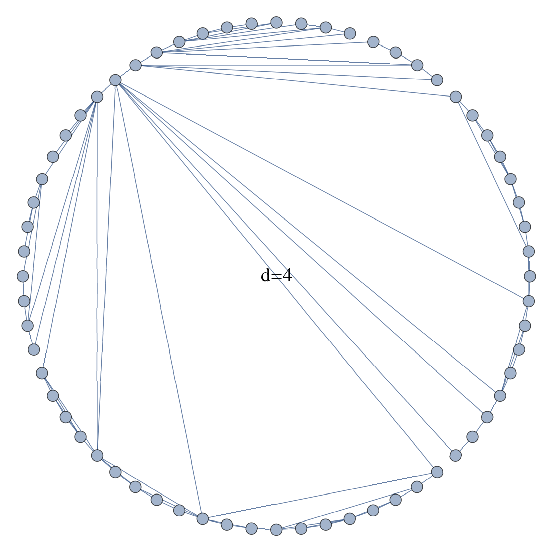
\includegraphics[width=180px]{h4.eps}
    \end{tabular}
    \caption{The degree distribution found in the numerical experiments (dots)
    and the corresponding fitted function $A k^{-\gamma}$ (solid line) for $d=4$. The dotted line
    representing $P_{rand}(k)= (1/3)(2/3)^{k-2}$ was included in the HV plot just for comparison.}
    \label{frame}
\end{figure}



\begin{figure}[h]
    \centering
    \begin{tabular}{cc}
         natural visibility & horizontal visibility \\
         \includegraphics[width=180px]{v5.eps}&\includegraphics[width=180px]{h5.eps}
    \end{tabular}
    \caption{The degree distribution found in the numerical experiments (dots)
    and the corresponding fitted function $A k^{-\gamma}$ (solid line) for $d=5$. The dotted line
    representing $P_{rand}(k)= (1/3)(2/3)^{k-2}$ was included in the HV plot just for comparison.}
    \label{frame}
\end{figure}



\begin{figure}[h]
    \centering
    \begin{tabular}{cc}
         natural visibility & horizontal visibility \\
         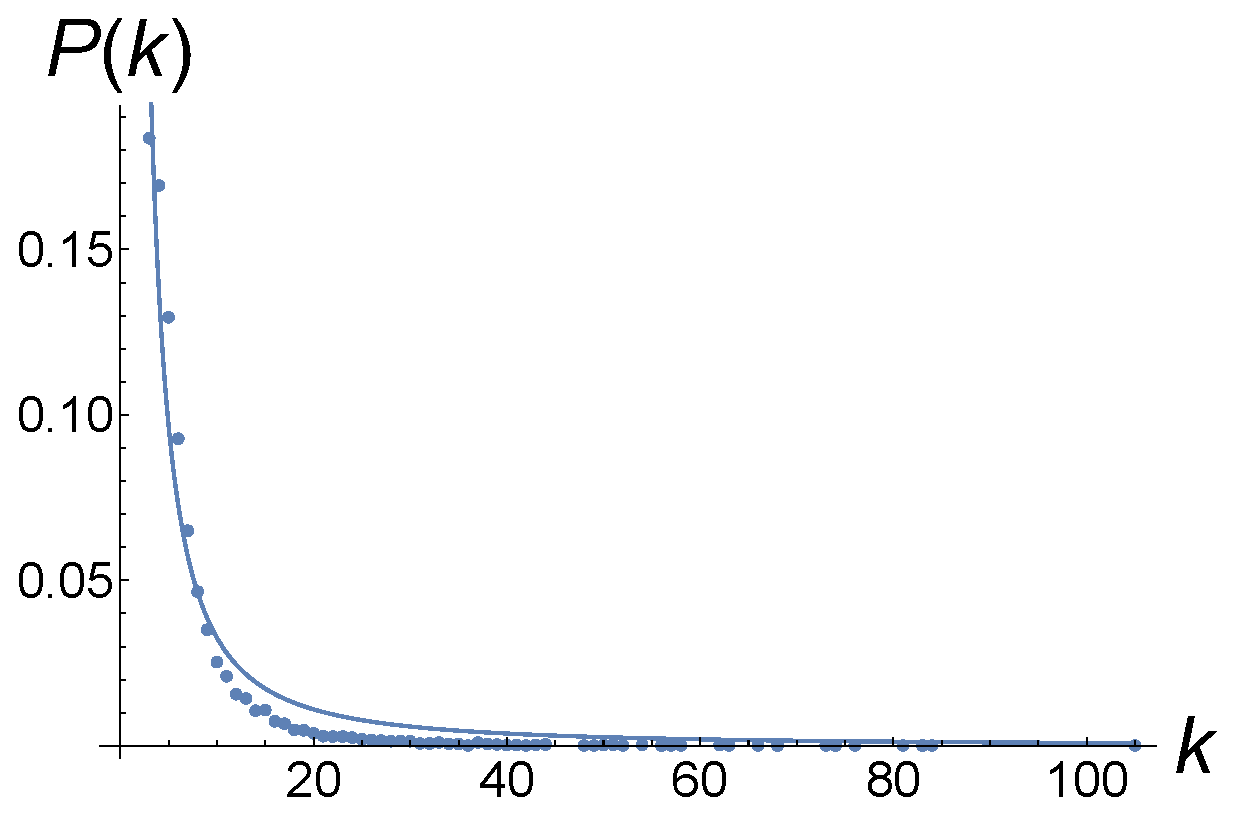
\includegraphics[width=180px]{vis4.eps}&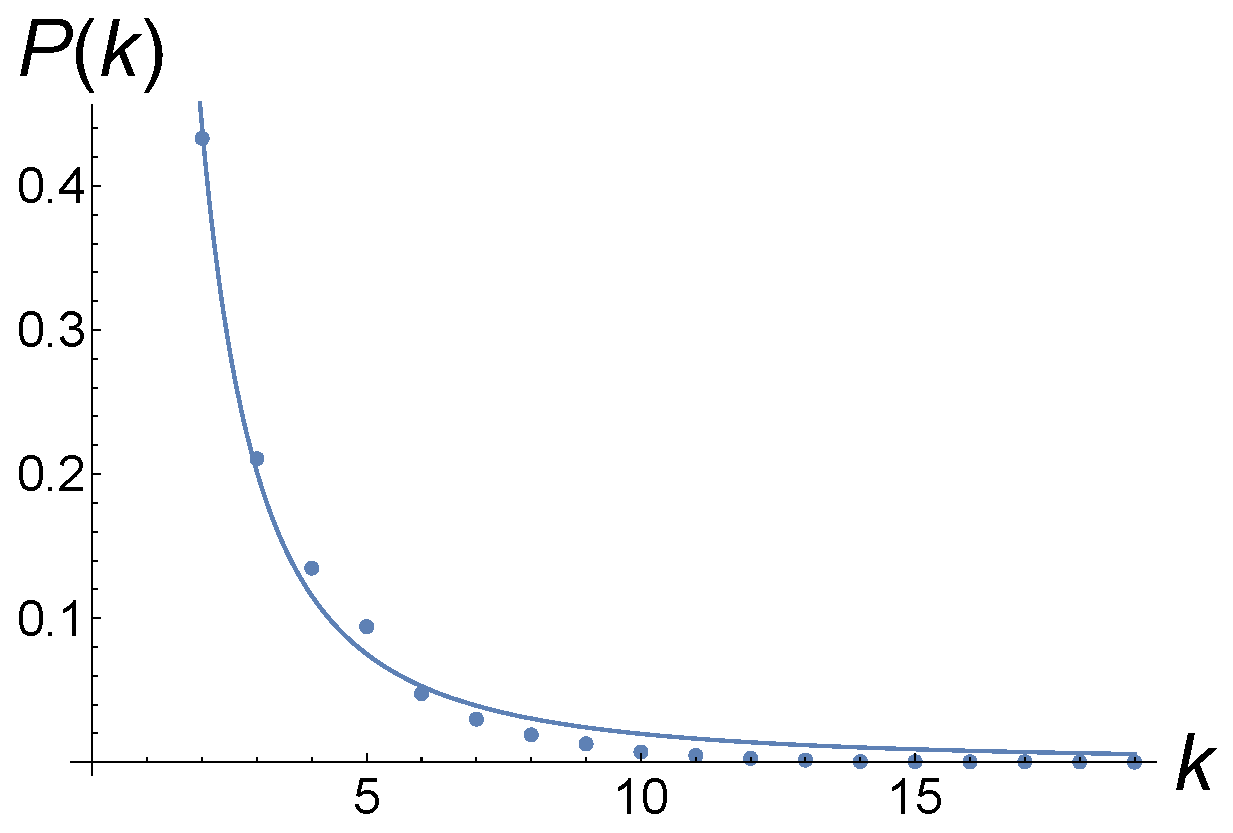
\includegraphics[width=180px]{hvis4.eps}
    \end{tabular}
    \caption{The degree distribution found in the numerical experiments (dots)
    and the corresponding fitted function $A k^{-\gamma}$ (solid line) for $d=4$.}
    \label{frame}
\end{figure}

\begin{figure}[h]
    \centering
    \begin{tabular}{cc}
         natural visibility & horizontal visibility \\
         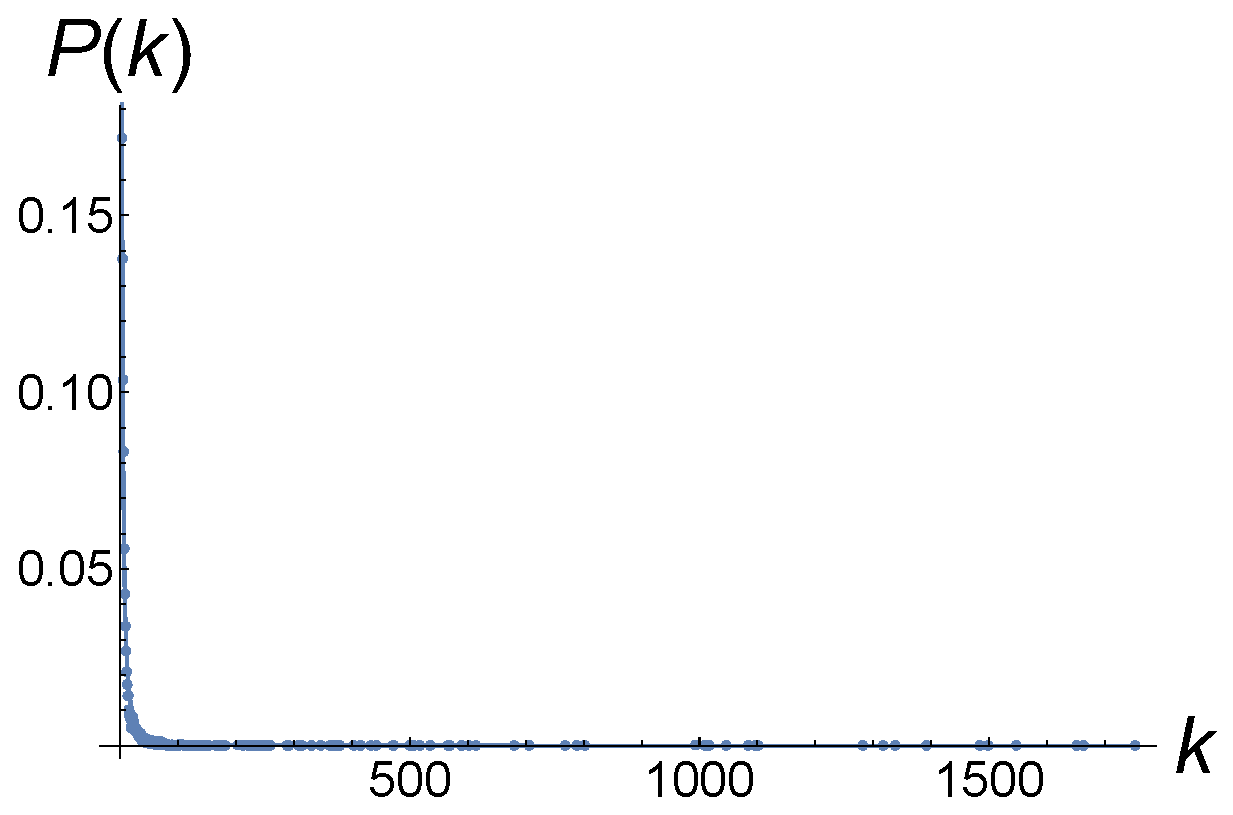
\includegraphics[width=180px]{vis5.eps}&\includegraphics[width=180px]{hvis5.eps}
    \end{tabular}
    \caption{The degree distribution found in the numerical experiments (dots)
    and the corresponding fitted function $A k^{-\gamma}$ (solid line) for $d=5$.}
    \label{frame}
\end{figure}

\begin{figure}[h]
    \centering
    \begin{tabular}{cc}
         natural visibility & horizontal visibility \\
         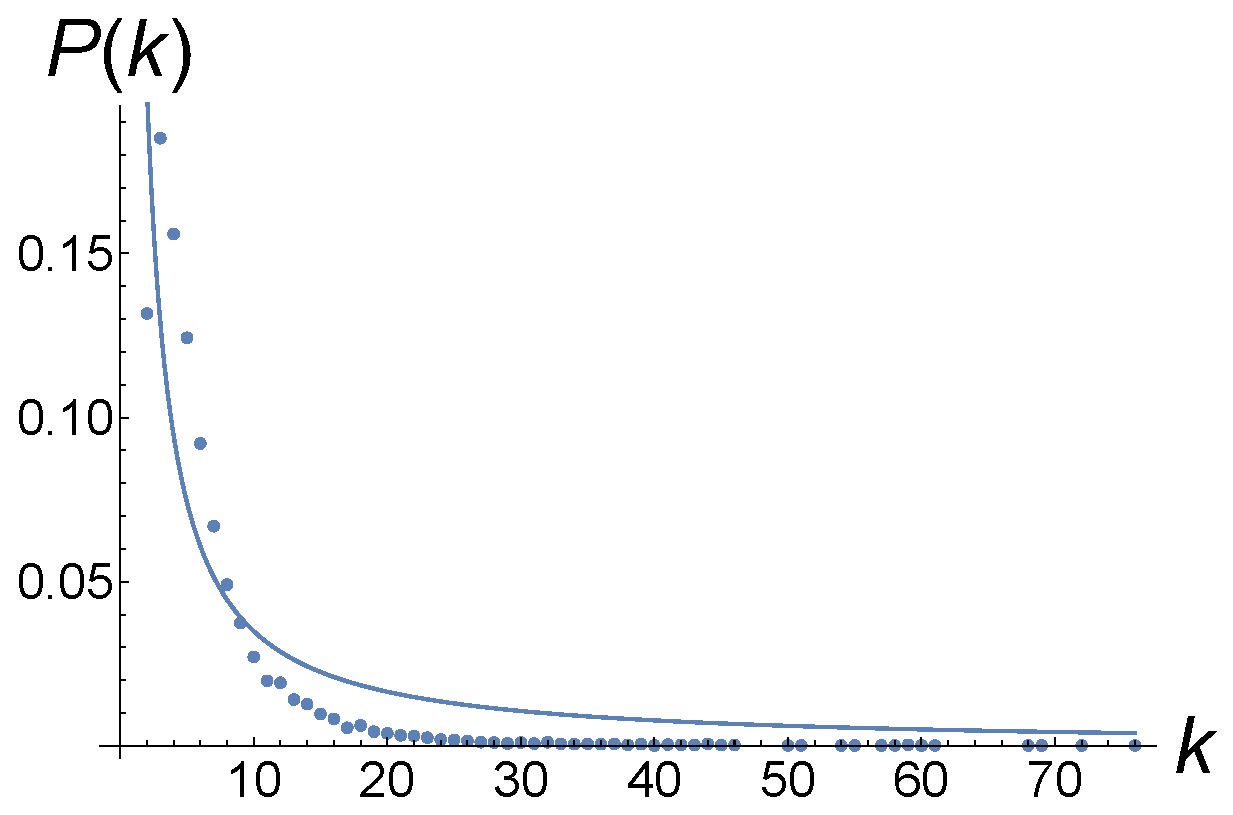
\includegraphics[width=180px]{vis6.eps}&\includegraphics[width=180px]{hvis6.eps}
    \end{tabular}
    \caption{The degree distribution found in the numerical experiments (dots)
    and the corresponding fitted function $A k^{-\gamma}$ (solid line) for $d=6$.}
    \label{frame}
\end{figure}

\end{document}

Prime distribution was also studied via binary images \cite{a01} and
from graphs. For instance, prime numbers can be converted into
graphs by breaking an even number as the sum of two primes. Two
primes, which are the nodes of this graph, are linked if they
compose such a sum \cite{a04}. In another graph in which the natural
numbers are the nodes, there is a connection between two nodes if
they share a common prime divisor \cite{a16}.

The distribution of prime numbers throughout the sequence of natural
numbers has been extensively investigated. Giants as Chebyshev,
Dirichlet, Erd\"os, Euclid, Euler, Fermat, Legendre, Gauss, and
Riemann analytically studied this matter \cite{a44,a66}. In the last
decades, the statistical properties of the gaps between consecutive
primes \cite{a64,a03}, second order gaps (the gaps between these
gaps), and higher order gaps \cite{a05} have been examined. Also,
spectral analyses of these gaps \cite{a02} and of the amount of
primes inside subintervals of the domain of positive integers
\cite{a09} were already performed \cite{a02}. Prime distribution was
also studied via binary images of such numbers \cite{a01} and from
graphs. For instance, prime numbers can be converted into graphs by
breaking an even number as the sum of two primes. Two primes, which
are the nodes of this graph, are linked if they compose such a sum
\cite{a04}. In another graph in which the natural numbers are the
nodes, there is a connection between two nodes if they share a
common prime divisor \cite{a16}.

Thus, weakly connected nodes are more frequent that highly connected
nodes.


Thus, a small subset of ''high" differences (''high" values of
$x_d$) are highly connected and a high subset of ''small"
differences are

A power-law distribution in the connectivity of complex networks can
be (easily) generated by a variety of mechanisms (such as
preferential attachment rule \cite{a81,a83}). This distribution was
found in the networks derived from $d$-primes, suggesting that


Advances in Mathematical Physics Volume 2011, Article ID 519178, 8
pages doi:10.1155/2011/519178 Research Article Hidden Periodicity
and Chaos in the Sequence of Prime Numbers A. Bershadskii
